%% beamer packages
% other themes: AnnArbor, Antibes, Bergen, Berkeley, Berlin, Boadilla, boxes, 
% CambridgeUS, Darmstadt, Dresden, Frankfurt, Goettingen, Hannover, Ilmenau,
%JuanLesPins, Luebeck, Madrid, Malmoe, Marburg, Montpellier, PaloAlto,
%Pittsburgh, Rochester, Singapore, Szeged, Warsaw
% other colors: albatross, beaver, crane, default, dolphin, dove, fly, lily, 
%orchid, rose, seagull, seahorse, sidebartab, structure, whale, wolverine,
%beetle

%\documentclass[xcolor=dvipsnames]{beamer}
\documentclass[table,dvipsnames]{beamer}
\usepackage{beamerthemesplit}
\usepackage{bm,amsmath,marvosym}
\usepackage{listings,color}%xcolor
\usepackage[ngerman]{babel}
\usepackage{natbib}
\usepackage[utf8]{inputenc}
\definecolor{shadecolor}{rgb}{.9, .9, .9}
\definecolor{darkblue}{rgb}{0.0,0.0,0.5}
\definecolor{myorange}{cmyk}{0,0.7,1,0}
\definecolor{mypurple}{cmyk}{0.3, 0.9, 0.0, 0.2}

% make a checkmark
\usepackage{tikz}
\def\checkmark{\tikz\fill[scale=0.4](0,.35) -- (.25,0) -- (1,.7) -- (.25,.15) -- cycle;} 

% dot product
\usetikzlibrary{arrows,positioning}
\tikzset{
    %Define standard arrow tip
    >=stealth',
    % Define arrow style
    pil/.style={->,thick}
}

% math stuff
\newcommand{\argmin}{\operatornamewithlimits{argmin}}

\lstnewenvironment{code}{
    \lstset{backgroundcolor=\color{shadecolor},
        showstringspaces=false,
        language=python,
        frame=single,
        framerule=0pt,
        keepspaces=true,
        breaklines=true,
        basicstyle=\ttfamily,
        keywordstyle=\bfseries,
        basicstyle=\ttfamily\scriptsize,
        keywordstyle=\color{blue}\ttfamily,
        stringstyle=\color{red}\ttfamily,
        commentstyle=\color{green}\ttfamily,
        columns=fullflexible
    }
}{}

\lstnewenvironment{codeout}{
    \lstset{backgroundcolor=\color{shadecolor},
        frame=single,
        framerule=0pt,
        breaklines=true,
        basicstyle=\ttfamily\scriptsize,
        columns=fullflexible
    }
}{}

\hypersetup{colorlinks = true, linkcolor=darkblue, citecolor=darkblue,urlcolor=darkblue}
\hypersetup{pdfauthor={A. Richards}, pdftitle={Intro to probabilistic programming}}

\newcommand{\rd}{\textcolor{red}}
\newcommand{\grn}{\textcolor{green}}
\newcommand{\keywd}{\textcolor{myorange}}
\newcommand{\highlt}{\textcolor{NavyBlue}}
\newcommand{\norm}[1]{\left\lVert#1\right\rVert}
\def\ci{\perp\!\!\!\perp}
% set beamer theme and color
\usetheme{Frankfurt}
%\usetheme{Berkeley}
\usecolortheme{orchid}
%\usecolortheme{seagull}

%% modify the font
%\usepackage{fontspec}
%setting a font
%\setsansfont{TeX Gyre Adventor}
%\usepackage{newcent}

%% fix the section title for literature
\renewcommand{\bibsection}{\subsubsection*{\bibname } }

\title[Project teams]{Introduction to probabilistic programming \\ (with PyMC3)}
\author[A. Richards]{A. Richards}
\institute{}
\date[]{02.08.2017}

%%%%%%%%%%%%%%%%%%%%%%%%%%%%%%%%%%%%%%%%%%%%%%%%%%%%%%%%%%%%%%%%%%%%%%%%%%%%%%%
\begin{document}
\frame{\titlepage}
%%%%%%%%%%%%%%%%%%%%%%%%%%%%%%%%%%%%%%%%%%%%%%%%%%%%%%%%%%%%%%%%%%%%%%%%%%%%%%%
\frame{
\footnotesize
\tableofcontents
\normalsize
}

%%%%%%%%%%%%%%%%%%%%%%%%%%%%%%%%%%%%%%%%%%%%%%%%%%%%%%%%%%%%%%%%%%%%%%%%%%%%%%%
\section{Introduction}
\subsection{}
%%%%%%%%%%%%%%%%%%%%%%%%%%%%%%%%%%%%%%%%%%%%%%%%%%%%%%%%%%%%%%%%%%%%%%%%%%%%%%%
\frame{   
\frametitle{Probabilistic programming}
\footnotesize
\begin{block}{A probabilistic programming language makes it easy to:}
 \begin{enumerate}
  \item write out complex probability models
  \item And subsequently solve these models automatically.
 \end{enumerate}
 \end{block}

\begin{block}{Generally this is accomplished by:}
 \begin{enumerate}
  \item Random variables are handled as a \href{https://en.wikipedia.org/wiki/Language\_primitive}{primitive}
  \item Inference is handled behind the scenes
  \item Memory and processor management is abstracted away
 \end{enumerate}
 \end{block} 
}

%%%%%%%%%%%%%%%%%%%%%%%%%%%%%%%%%%%%%%%%%%%%%%%%%%%%%%%%%%%%%%%%%%%%%%%%%%%%%%%
\frame{ 
\frametitle{The pros and the cons}
\footnotesize
\textbf{Why you might want to use probabilistic programming}
\begin{enumerate}
 \item \keywd{Customization} - We can create models that have built-in hypothesis tests
 \item \keywd{Propagation of uncertainty} - There is a degree of belief associated prediction and estimation
 \item \keywd{Intuition} - The models are essentially 'white-box' which provides insight into our data
\end{enumerate}
\textbf{Why you might \highlt{NOT} want use out probabilistic programming}
\begin{enumerate}
 \item \keywd{Deep dive} - Many of the online examples will assume a fairly deep understanding of statistics
 \item \keywd{Overhead} - Computational overhead might make it difficult to be production ready
 \item \keywd{Sometimes simple is enough} - The ability to customize models in almost a plug-n-play manner has to come with some cost. 
\end{enumerate}
}

%%%%%%%%%%%%%%%%%%%%%%%%%%%%%%%%%%%%%%%%%%%%%%%%%%%%%%%%%%%%%%%%%%%%%%%%%%%%%%%
\frame{ 
\frametitle{Bayesian Inference}
\large \highlt{Degree of belief} \\ \ \\
\footnotesize
You are a skilled programmer, but bugs still slip into your code. After a particularly difficult implementation of an algorithm, you decide to test your code on a trivial example. It passes. You test the code on a harder problem. It passes once again. And it passes the next, \textit{even more difficult}, test too! You are \highlt{starting to believe} that there may be no bugs in this code...

\begin{flushleft}
\href{https://github.com/CamDavidsonPilon/Probabilistic-Programming-and-Bayesian-Methods-for-Hackers}{Bayesian methods for hackers}
\end{flushleft}

This is \href{http://www.kdnuggets.com/2016/12/datascience-introduction-bayesian-inference.html}{a nice intro to Bayesian thinking done on kdnuggets (using PyMC3)}
}

%%%%%%%%%%%%%%%%%%%%%%%%%%%%%%%%%%%%%%%%%%%%%%%%%%%%%%%%%%%%%%%%%%%%%%%%%%%%%%%
\frame{ 
\frametitle{Some terminology}
\footnotesize
\begin{equation}
P(\theta|x) = \frac{P(x|\theta)P(\theta)}{P(x)}
\end{equation}

\begin{itemize}
 \item \keywd{prior} - $P(\theta)$ - one's beliefs about a quantity before presented with evidence
 \item \keywd{posterior} - $P(\theta|x)$ - probability of the parameters given the evidence
 \item \keywd{likelihood} - $P(x|\theta)$  - probability of the evidence given the parameters
 \item \keywd{normalizing constant} - $P(x)$
\end{itemize}

\begin{itemize}
 \item $P(\theta)$: This big, complex code likely has a bug in it. 
 \item $P(\theta|X)$: The code passed all X tests; there still might be a bug, but it is less likely now.
\end{itemize}
}

%%%%%%%%%%%%%%%%%%%%%%%%%%%%%%%%%%%%%%%%%%%%%%%%%%%%%%%%%%%%%%%%%%%%%%%%%%%%%%%%
\frame{
\begin{center}
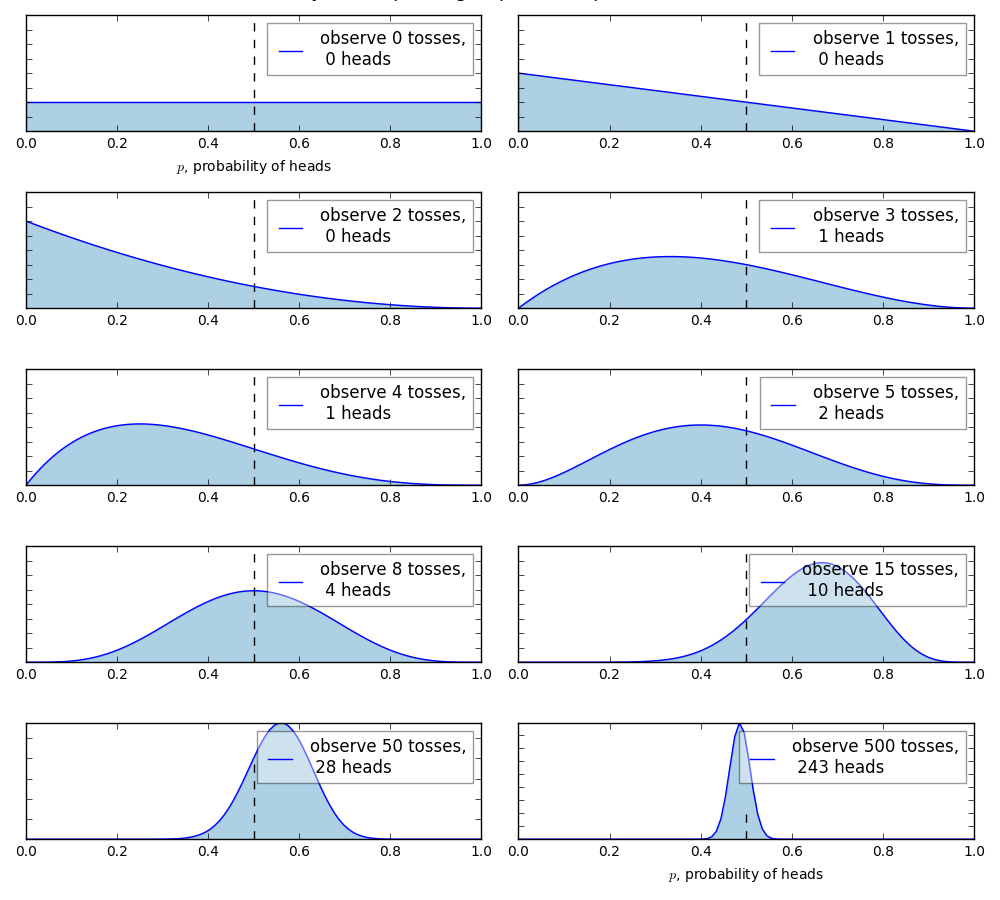
\includegraphics[scale=0.32]{coin_flip.png}
\end{center}
}

%%%%%%%%%%%%%%%%%%%%%%%%%%%%%%%%%%%%%%%%%%%%%%%%%%%%%%%%%%%%%%%%%%%%%%%%%%%%%%%
\section{Warm up}
\subsection{}
%%%%%%%%%%%%%%%%%%%%%%%%%%%%%%%%%%%%%%%%%%%%%%%%%%%%%%%%%%%%%%%%%%%%%%%%%%%%%%%

%%%%%%%%%%%%%%%%%%%%%%%%%%%%%%%%%%%%%%%%%%%%%%%%%%%%%%%%%%%%%%%%%%%%%%%%%%%%%%%
\begin{frame}[fragile]
\frametitle{PyMC3}
\footnotesize
\begin{code}
import pymc3 as pm
\end{code}

\begin{itemize}
 \item Developed by John Salvatier, Thomas Wiecki, and Christopher Fonnesbeck \citep{Salvatier16}
 \item Comes with \href{https://github.com/pymc-devs/pymc3/tree/master/pymc3/examples}{loads of good examples}
 \item API is is not backwards compartible with models specified in PyMC2
 \item Can still be run in Python2.7+.
\end{itemize}

\highlt{Basic workflow}
\begin{enumerate}
 \item Define hyperpriors
 \item Open a model context
 \item Perform inference
\end{enumerate}
\end{frame}

%%%%%%%%%%%%%%%%%%%%%%%%%%%%%%%%%%%%%%%%%%%%%%%%%%%%%%%%%%%%%%%%%%%%%%%%%%%%%%%
\frame{
\frametitle{Markov chain Monte Carlo (MCMC)}
\footnotesize
\keywd{MCMC}
\begin{itemize}
 \item It is an family of algorithms for obtaining a sequence of random samples from a probability distribution for which direct sampling is difficult.
 \item The sequence can then be used to approximate the distribution
 \item It allows for inference on complex models
\end{itemize}

A particularly useful class of MCMC, known as Hamliltonian Monte Carlo, requires \href{https://en.wikipedia.org/wiki/Gradient}{gradient} information which is often not readily available so PyMC3 uses Theano to get around this problem.  Something that has recently made this whole field a lot more interesting is the No-U-turn sampler (NUTS) because there are \highlt{self-tuning strategies} \citep{Hoffman14}.
\\ \ \\
One of the really nice things about probabilistic programming is that \highlt{you do not have to know how inference is performed}, but it can be useful.  

\begin{itemize}
 \item \href{http://twiecki.github.io/blog/2015/11/10/mcmc-sampling/}{MCMC for Dummies}
 \item \href{https://arxiv.org/pdf/1206.1901.pdf}{More on Hamliltonian MCMC (Not for dummies)}
 \item \href{http://twiecki.github.io/blog/2014/01/02/visualizing-mcmc/}{How to animate MCMC (for everyone)}
\end{itemize}
}

%%%%%%%%%%%%%%%%%%%%%%%%%%%%%%%%%%%%%%%%%%%%%%%%%%%%%%%%%%%%%%%%%%%%%%%%%%%%%%%
\begin{frame}[fragile]
\begin{block}{PyMC3 is an improvement over PyMC2}
\begin{itemize}
 \item Intuitive model specification syntax e.g. \\
 \begin{equation*}
 x \sim N(0,1) \textrm{ becomes } x = \textrm{Normal}(0,1)
 \end{equation*}
 \item Powerful sampling algorithms such as the \href{http://arxiv.org/abs/1111.4246}{No U-Turn Sampler}
 \item \highlt{Variational inference}: \href{http://arxiv.org/abs/1506.03431}{ADVI} for fast approximate posterior estimation as well as \highlt{mini-batch} ADVI for large data sets.
 \item Relies on \href{http://deeplearning.net/software/theano}{Theano} which provides:
 \begin{itemize}
 \item Numpy broadcasting and advanced indexing
 \item Linear algebra operators
 \item Computation optimization and dynamic C compilation
 \item Simple extensibility
 \end{itemize}
 \item Transparent support for \highlt{missing value imputation}
\end{itemize}
\end{block}
\end{frame}

%%%%%%%%%%%%%%%%%%%%%%%%%%%%%%%%%%%%%%%%%%%%%%%%%%%%%%%%%%%%%%%%%%%%%%%%%%%%%%%
\frame{ 
\frametitle{Getting started}
\footnotesize

\begin{block}{}
 We will be using probabilistic programming with PyMC3 to perform automatic Bayesian inference on user-defined probabilistic models
\end{block}
\vspace{0.5cm	}
These are some of the best getting started resources out there
\begin{itemize}
 \item \href{https://github.com/pymc-devs/pymc3}{PyMC3 repo}
 \item \href{http://pymc-devs.github.io/pymc3/notebooks/getting_started.html}{Getting started guide}
 \item \href{https://github.com/CamDavidsonPilon/Probabilistic-Programming-and-Bayesian-Methods-for-Hackers}{Bayesian methods for hackers}
\end{itemize}
\vspace{0.5cm}
Now that we have an intuition for Bayesian inference and a general idea of what to expect with PyMC3 lets dive in.
}

%%%%%%%%%%%%%%%%%%%%%%%%%%%%%%%%%%%%%%%%%%%%%%%%%%%%%%%%%%%%%%%%%%%%%%%%%%%%%%%
\begin{frame}[fragile]
\frametitle{PyMC3}
\footnotesize
\begin{code}
import pymc3 as pm

n,h,alpha,beta,niter = 100,61,2,2,1000

# context management
with pm.Model() as model: 
    p = pm.Beta('p', alpha=alpha, beta=beta)
    y = pm.Binomial('y', n=n, p=p, observed=h)

    start = pm.find_MAP()
    step = pm.Metropolis()
    trace = pm.sample(niter, step, start)
\end{code}

Data $\rightarrow$ Model context $\rightarrow$ Priors $\rightarrow$ Likelihood $\rightarrow$ Sampler $\rightarrow$ Inference
\vspace{0.5cm}
\\ \noindent To the notebooks!
\end{frame}

%%%%%%%%%%%%%%%%%%%%%%%%%%%%%%%%%%%%%%%%%%%%%%%%%%%%%%%%%%%%%%%%%%%%%%%%%%%%%%%
\frame{   
\frametitle{Where are we...}
\begin{block}{}
 \begin{itemize}
  \item[\checkmark] Overview
  \item[\checkmark] Coin-flip example
  \item[\checkmark] Estimating the mean and standard deviation of a Normal
  \item[\checkmark] Switchpoint analysis of text messages
  \end{itemize}
\end{block}
}

%%%%%%%%%%%%%%%%%%%%%%%%%%%%%%%%%%%%%%%%%%%%%%%%%%%%%%%%%%%%%%%%%%%%%%%%%%%%%%%
\begin{frame}[fragile]
\frametitle{There are more examples..}
\begin{block}{}
 But what about linear regression--the classical example??
\end{block}

The linear regression example \href{http://pymc-devs.github.io/pymc3/notebooks/getting_started.html}{is well explained in the docs}, but I did want to point out that we now have access to GLM style formulations in PyMC3.
\vspace{1cm}
\begin{code}
import pymc3 as pm

...

data = dict(x=x, y=y)

with pm.Model() as model:
    pm.glm.glm('y ~ x', data)
    step = pm.NUTS()
    trace = pm.sample(2000, step, progressbar=True)
\end{code}    
\end{frame}
%%%%%%%%%%%%%%%%%%%%%%%%%%%%%%%%%%%%%%%%%%%%%%%%%%%%%%%%%%%%%%%%%%%%%%%%%%%%%%%
\section{PMF}
\subsection{}
%%%%%%%%%%%%%%%%%%%%%%%%%%%%%%%%%%%%%%%%%%%%%%%%%%%%%%%%%%%%%%%%%%%%%%%%%%%%%%%

%%%%%%%%%%%%%%%%%%%%%%%%%%%%%%%%%%%%%%%%%%%%%%%%%%%%%%%%%%%%%%%%%%%%%%%%%%%%%%%
\frame{ 
\frametitle{Recommenders}

\begin{table}
\begin{center}
What will a user \textit{buy}, \textit{click}, \textit{like}...
\end{center}
\ \\ \ \\
\begin{tabular}{|l|c|c|c|c|c|c|c|c|}
\hline
        & A  &  B & C & D & E & F & G & ... \\
\hline        
Frodo   & 1  &  ? & 2 & 1 & 1 & 4 & 1 & ... \\
Sam     & ?  &  ? & 1 & 3 & ? & 3 & 1 & ... \\
Merry   & ?  &  ? & 1 & 1 & ? & 1 & 1 & ... \\
Gimli   & 1  &  1 & ? & 1 & ? & 1 & ? & ... \\
Legolas & 1  &  1 & ? & 1 & ? & 1 & ? & ... \\
\hline
\end{tabular}
\end{table}

\begin{itemize}
 \item Ebay and Amazon who recommends items for purchase
 \item Movies, dating services, social network feeds, recipes, jokes, hikes, ...
\end{itemize}
}

%%%%%%%%%%%%%%%%%%%%%%%%%%%%%%%%%%%%%%%%%%%%%%%%%%%%%%%%%%%%%%%%%%%%%%%%%%%%%%%
\frame{ 
\footnotesize

There are numerous types of recommender systems
\begin{itemize}
 \item \keywd{Popularity} - Most viewed, most well-liked, not customized to users
 \item \keywd{User-User} - Recommend items liked by users with similar results
 \item \keywd{Item-Item} - Recommend items similar to what the current user rated favorably
 \item \keywd{Matrix-Factorization} - Estimate a users underlying preferences
\end{itemize}
-------------------------------------------------------------------------------- \\
Two of the most commonly implemented varieties are:
\begin{itemize}
 \item \keywd{collaborative filtering} - Imagine that user 1 and user 2 both like the same 4 science fiction novels we can then infer that if user 1 also likes another similar novel then user 2 will have a good chance of also liking it.
 \item \keywd{Content-based recommender} - These systems also make use of extra features associated with the user
\end{itemize}
}

%%%%%%%%%%%%%%%%%%%%%%%%%%%%%%%%%%%%%%%%%%%%%%%%%%%%%%%%%%%%%%%%%%%%%%%%%%%%%%%
\frame{ 
\frametitle{Probabilistic matrix factorization (PMF)}
\footnotesize
\begin{itemize}
 \item Probabilistic approach to the collaborative filtering problem that takes a Bayesian perspective \citep{Salakhutdinov08}.
 \item The ratings $R$ are modeled as draws from a Gaussian distribution
 \item We use precision $\alpha$, a fixed parameter, that reflects the uncertainty of the estimations; the normal distribution is commonly reparameterized in terms of precision, which is the inverse of the variance.
 \item small precision parameters help control the growth of our latent parameters
 \end{itemize}
The following implementation is modified from the \href{https://pymc-devs.github.io/pymc3/notebooks/pmf-pymc.html}{example in the PyMC3 documentation}.
\vspace{1cm}
Back to the notebook!
}

%%%%%%%%%%%%%%%%%%%%%%%%%%%%%%%%%%%%%%%%%%%%%%%%%%%%%%%%%%%%%%%%%%%%%%%%%%%%%%%
\frame{ 
\frametitle{Conclusions}
\footnotesize
\begin{itemize}
 \item Our results demonstrate that the mean of means method is our best baseline on our prediction task. 
 \item We are able to obtain a significant decrease in RMSE using the PMF MAP estimate obtained via Powell optimization. 
 \item We illustrated one way to monitor convergence of an MCMC sampler with a high-dimensionality sampling space 
 \item The traceplots using this method seem to indicate that our sampler converged to the posterior.
 \item Results using this posterior showed that attempting to improve the MAP estimation using MCMC sampling actually overfit the training data and increased test RMSE. This was likely caused by the constraining of the posterior via fixed precision parameters $\alpha$, $\alpha U$ and $\alpha V$.
\end{itemize}

\href{https://gist.github.com/macks22/00a17b1d374dfc267a9a}{this gist} is a working version of a fully Bayesian implementation.
}

%%%%%%%%%%%%%%%%%%%%%%%%%%%%%%%%%%%%%%%%%%%%%%%%%%%%%%%%%%%%%%%%%%%%%%%%%%%%%%%
\section{Cool down}
\subsection{}
%%%%%%%%%%%%%%%%%%%%%%%%%%%%%%%%%%%%%%%%%%%%%%%%%%%%%%%%%%%%%%%%%%%%%%%%%%%%%%%

%%%%%%%%%%%%%%%%%%%%%%%%%%%%%%%%%%%%%%%%%%%%%%%%%%%%%%%%%%%%%%%%%%%%%%%%%%%%%%%
\frame{ 
\frametitle{Neural Nets}
\begin{block}{Thomas Wiecki}
Has a \href{http://twiecki.github.io/blog/2016/06/01/bayesian-deep-learning/}{great blog post talking about exactly how to do this}
\end{block}

The notebook that is provided in this repo has not been significantly modified from  \href{https://github.com/twiecki/WhileMyMCMCGentlySamples/blob/master/content/downloads/notebooks/bayesian_neural_network.ipynb}{its original form}.  Although, check the original repository for the latest version.
}

%%%%%%%%%%%%%%%%%%%%%%%%%%%%%%%%%%%%%%%%%%%%%%%%%%%%%%%%%%%%%%%%%%%%%%%%%%%%%%%%
\frame{
\begin{center}
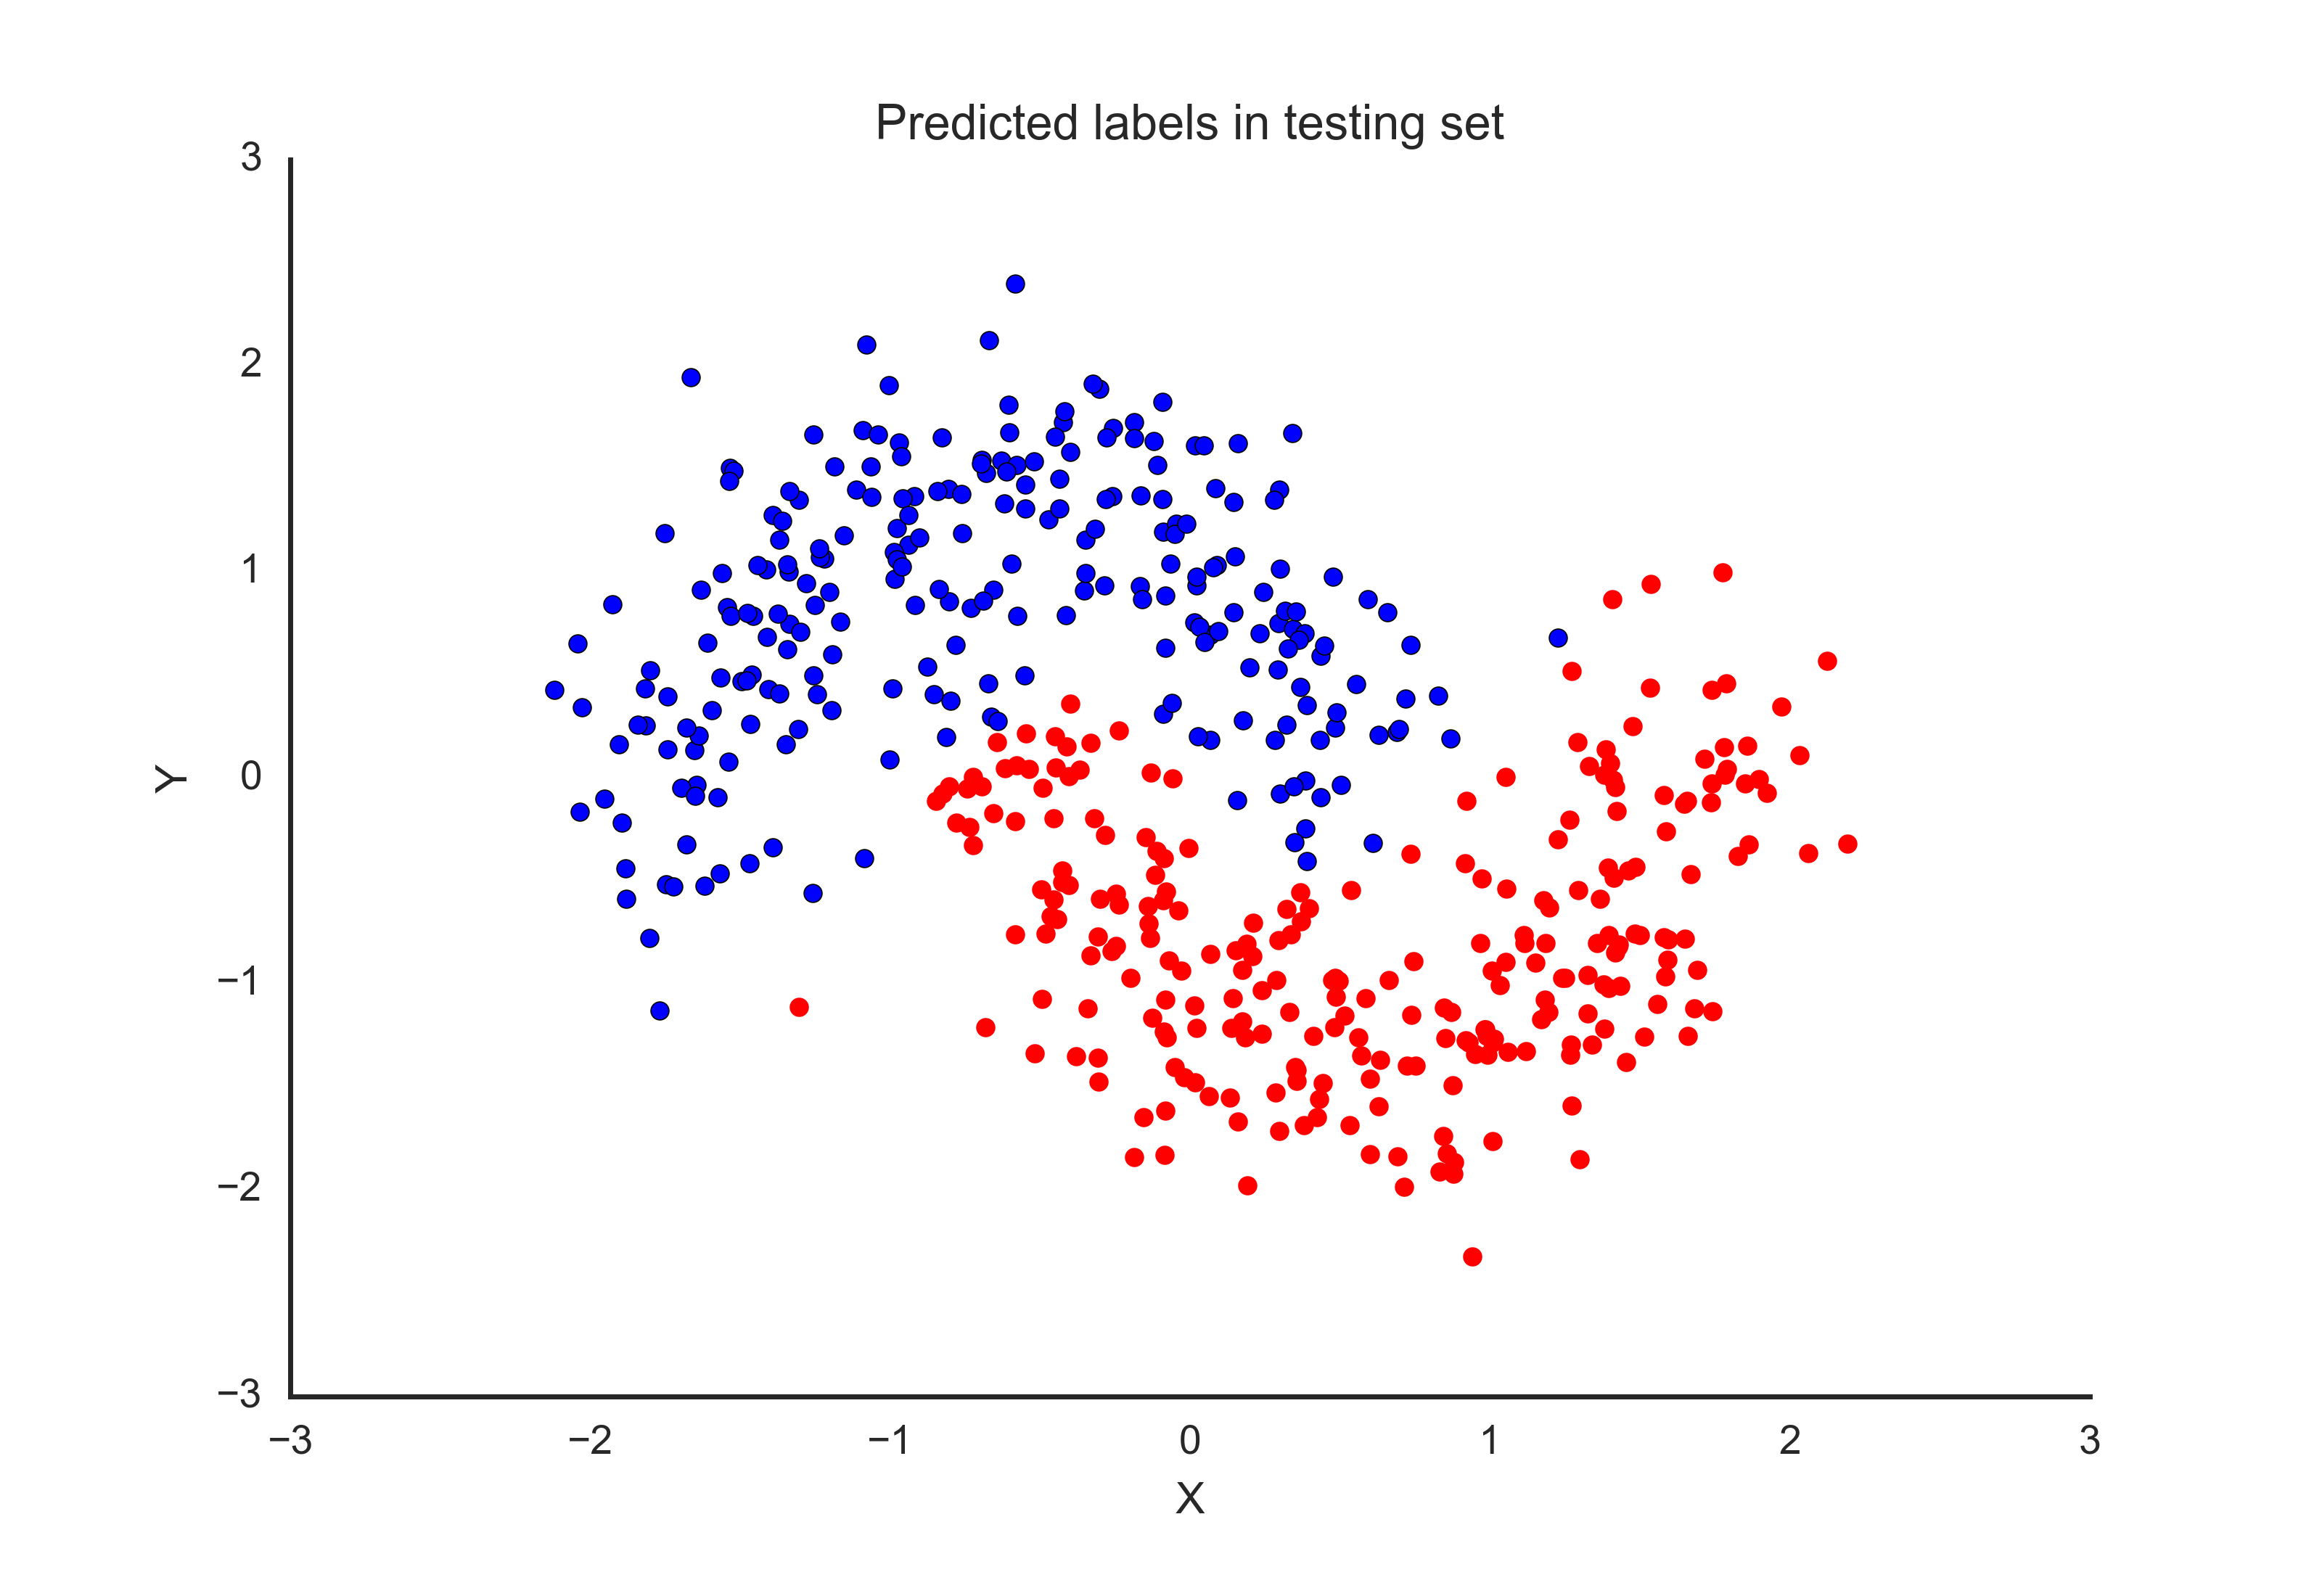
\includegraphics[scale=0.5]{../notebooks/nn-0.png}
\end{center}
}

%%%%%%%%%%%%%%%%%%%%%%%%%%%%%%%%%%%%%%%%%%%%%%%%%%%%%%%%%%%%%%%%%%%%%%%%%%%%%%%%
\frame{
\begin{center}
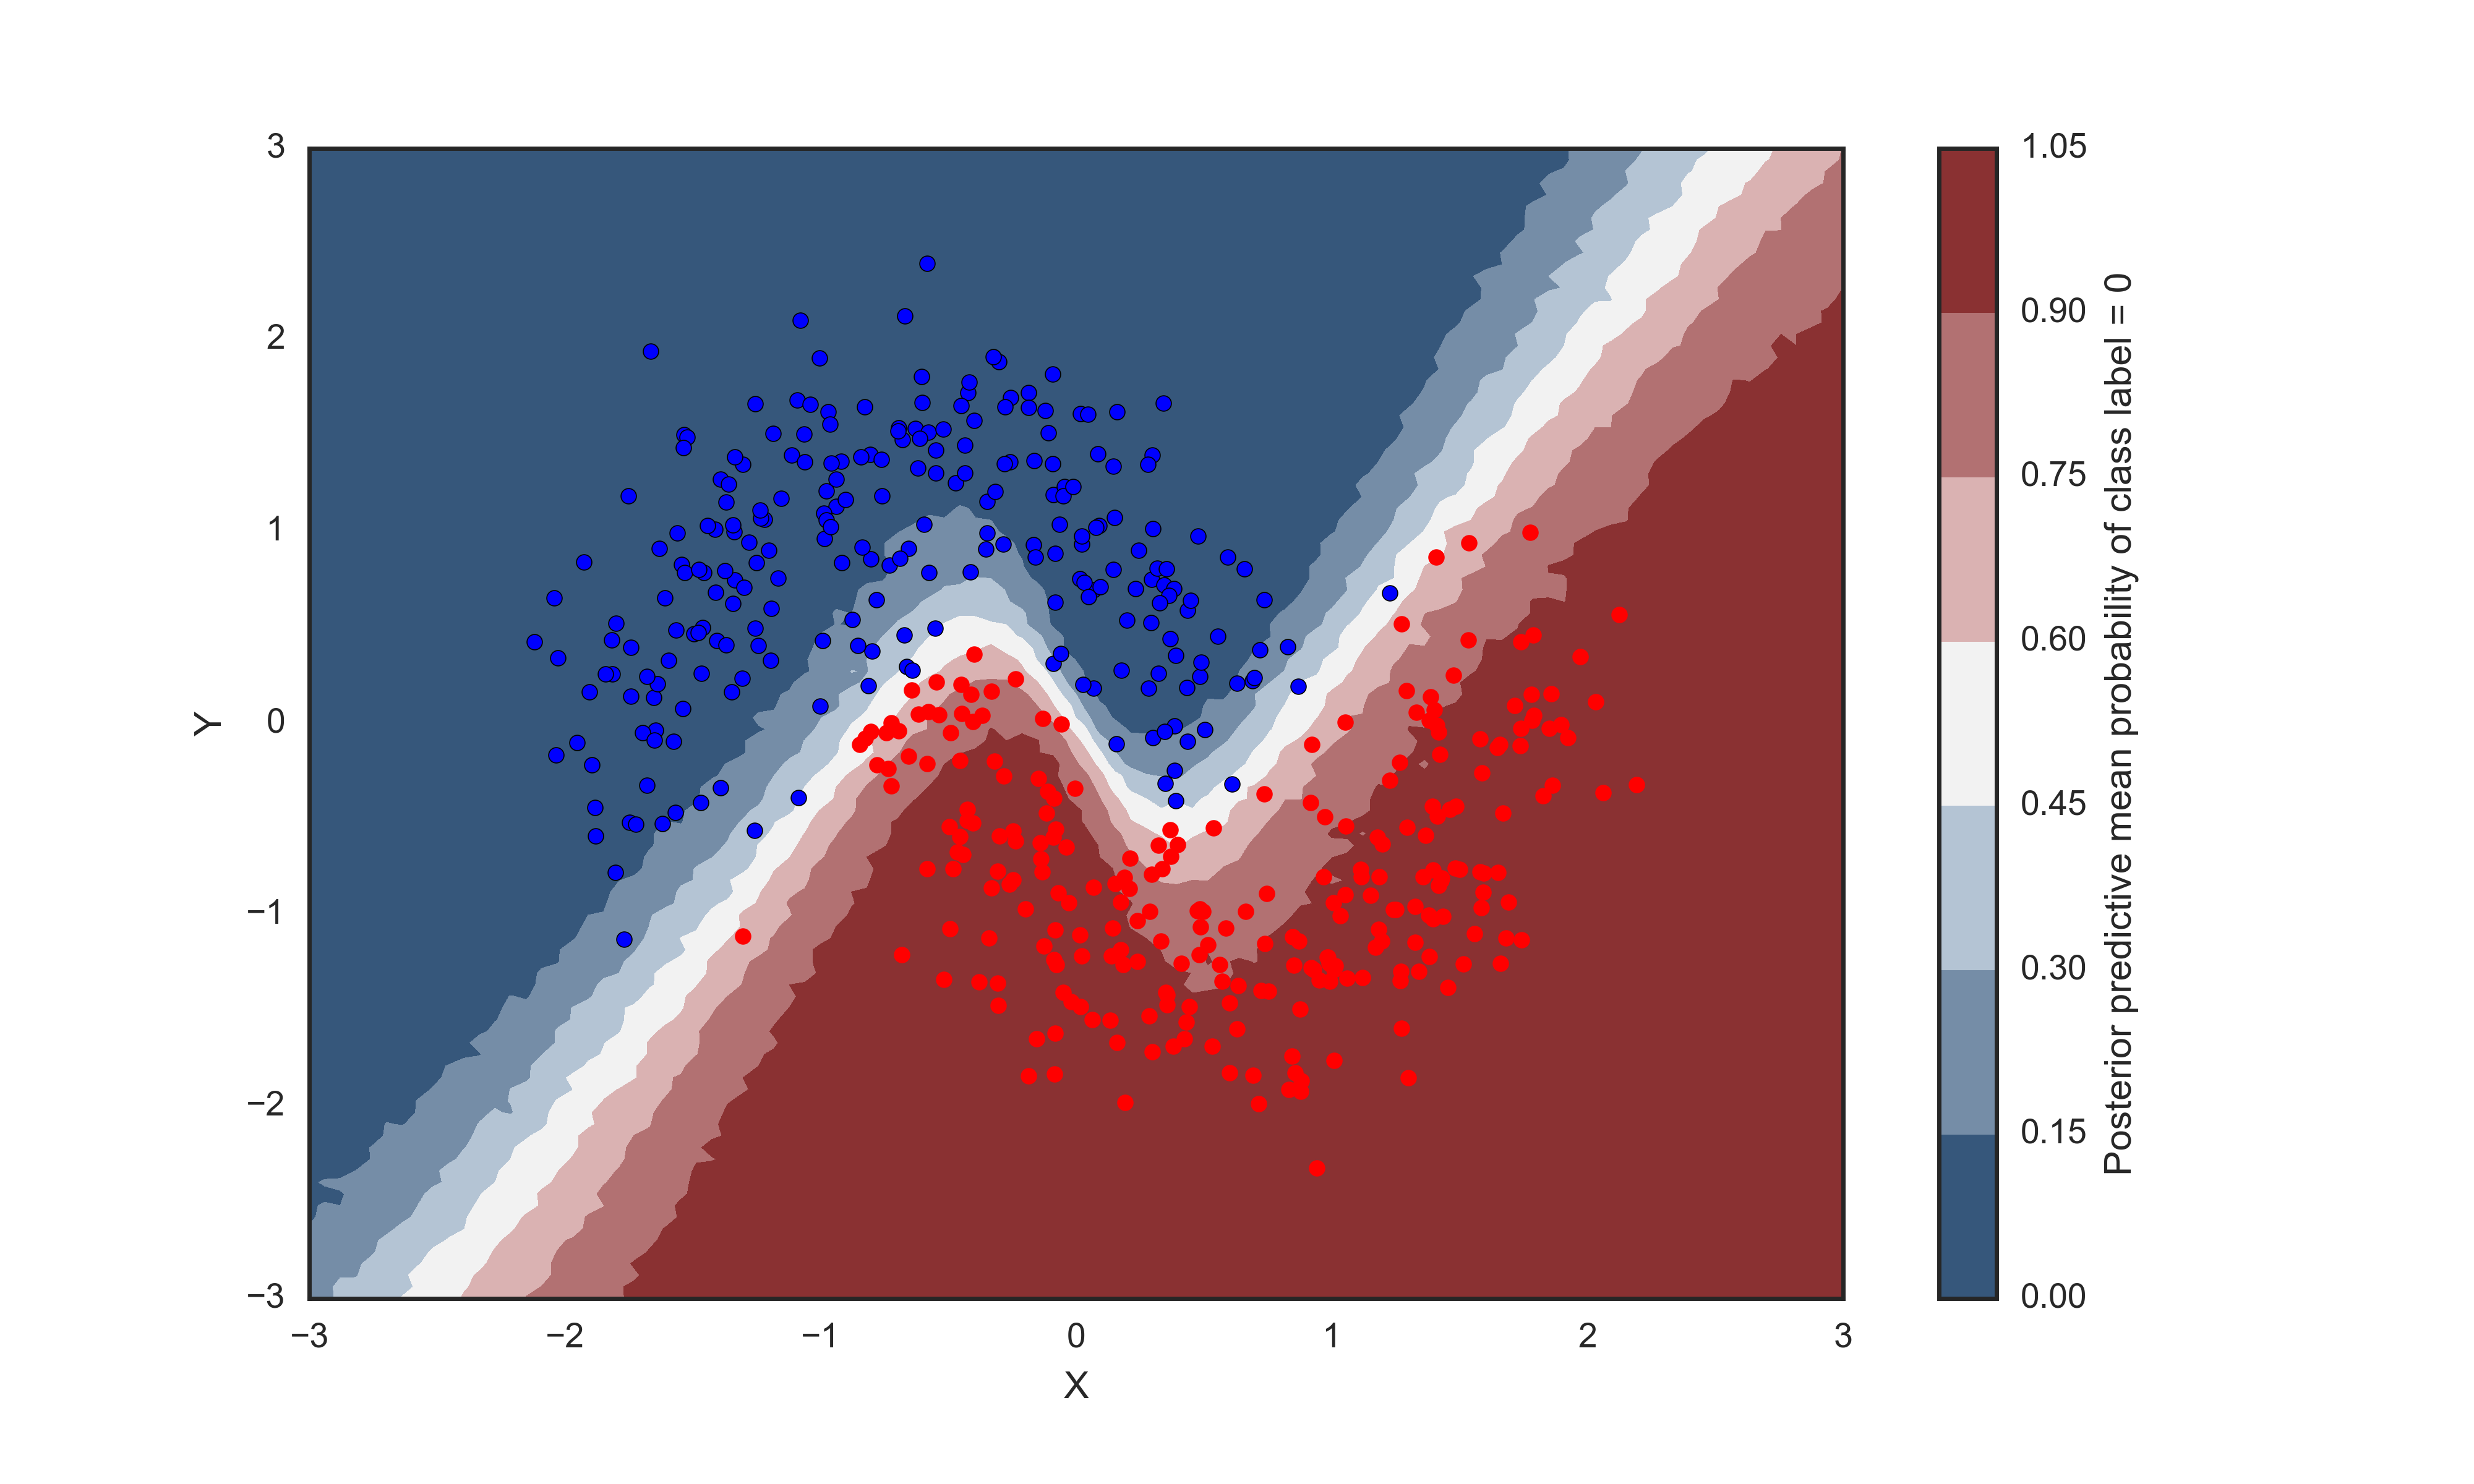
\includegraphics[scale=0.5]{../notebooks/nn-1.png}
\end{center}
}

%%%%%%%%%%%%%%%%%%%%%%%%%%%%%%%%%%%%%%%%%%%%%%%%%%%%%%%%%%%%%%%%%%%%%%%%%%%%%%%%
\frame{
\begin{center}
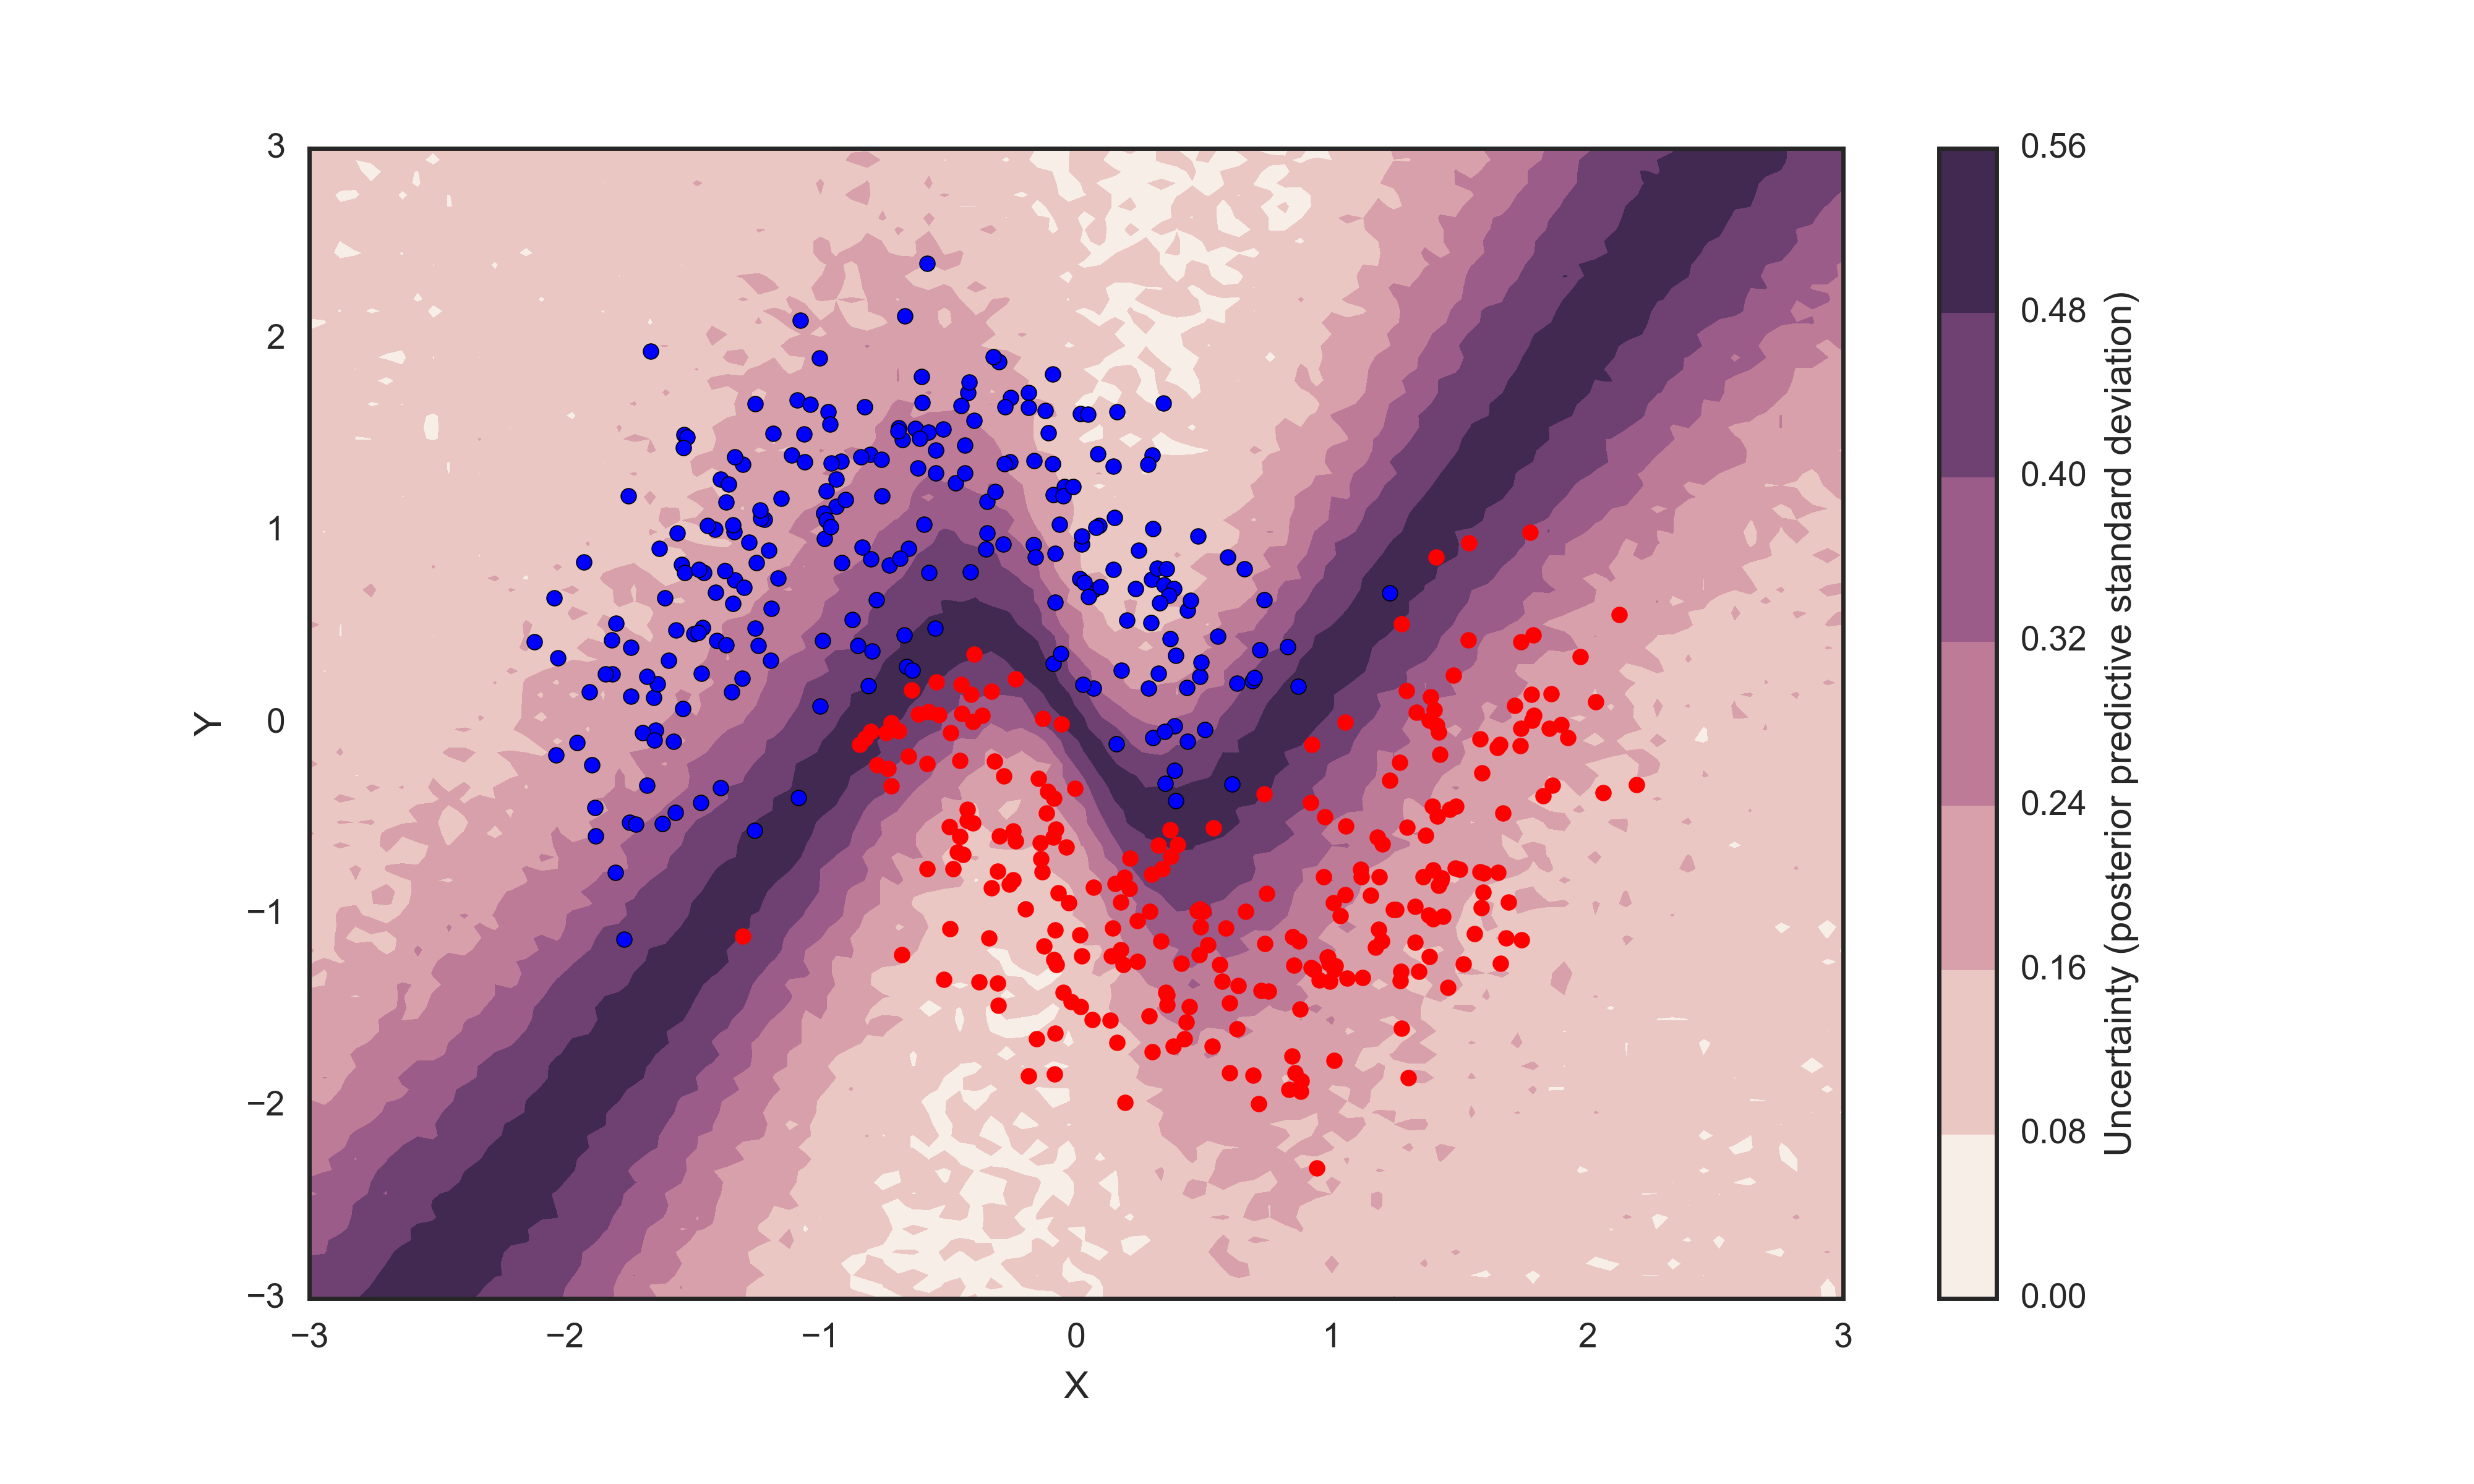
\includegraphics[scale=0.5]{../notebooks/nn-2.png}
\end{center}
}

%%%%%%%%%%%%%%%%%%%%%%%%%%%%%%%%%%%%%%%%%%%%%%%%%%%%%%%%%%%%%%%%%%%%%%%%%%%%%%%
\frame{ 
\frametitle{Another take on probabilistic programming}
\footnotesize
\begin{block}{}
 Another way of thinking about this: unlike a traditional program, which only runs in the forward directions, \highlt{a probabilistic program is run in both the forward and backward direction}. It runs forward to compute the consequences of the assumptions it contains about the world (i.e., the model space it represents), but it also runs backward from the data to constrain the possible explanations. In practice, many probabilistic programming systems will cleverly interleave these forward and backward operations to efficiently home in on the best explanations.
\end{block}
\vspace{1cm}
\href{https://plus.google.com/u/0/107971134877020469960/posts/KpeRdJKR6Z1}{Why Probabilistic Programming matters? (Beau Cronin)}
}

%%%%%%%%%%%%%%%%%%%%%%%%%%%%%%%%%%%%%%%%%%%%%%%%%%%%%%%%%%%%%%%%%%%%%%%%%%%%%%%
\frame{   
\frametitle{What did we cover again?}
\begin{block}{}
 \begin{itemize}
  \item[\checkmark] Overview
  \item[\checkmark] Coin-flip example
  \item[\checkmark] Estimating the mean and standard deviation of a Normal
  \item[\checkmark] Switchpoint analysis of text messages
  \item[\checkmark] Probabilistic matrix factorization
  \item[\checkmark] Probabilistic neural networks
  \end{itemize}
\end{block}
}

%%%%%%%%%%%%%%%%%%%%%%%%%%%%%%%%%%%%%%%%%%%%%%%%%%%%%%%%%%%%%%%%%%%%%%%%%%%%%%%
\frame{ 
\frametitle{Where to go from here}
\footnotesize

Examples, examples, examples...
\begin{itemize}
 \item \href{https://github.com/pymc-devs/pymc3}{PyMC3 repo}
 \item \href{http://pymc-devs.github.io/pymc3/notebooks/getting_started.html}{Getting started guide}
 \item \href{https://github.com/CamDavidsonPilon/Probabilistic-Programming-and-Bayesian-Methods-for-Hackers}{Bayesian methods 
for hackers}
  \item \href{http://twiecki.github.io}{Blog by Thomas Wiecki}
  \item \href{http://www.amazon.com/Doing-Bayesian-Analysis-Second-Edition/dp/0124058884/ref=dp_ob_title_bk}{Doing Bayesian Data Analysis by John Kruschke}
  \item \href{https://github.com/markdregan/Bayesian-Modelling-in-Python}{Resource by Mark Dregan}
\end{itemize}

There is also \href{https://github.com/stan-dev/example-models/wiki}{PyStan} (\href{http://www.stat.columbia.edu/~gelman/research/unpublished/stan-resubmit-JSS1293.pdf}{Stan paper})
}

%%%%%%%%%%%%%%%%%%%%%%%%%%%%%%%%%%%%%%%%%%%%%%%%%%%%%%%%%%%%%%%%%%%%%%%%%%%%%%
\frame[allowframebreaks]{  
\frametitle{References}
\begin{tiny} \bibliography{pp.bib}
\bibliographystyle{apalike}         % Style BST file
\end{tiny}
}

\end{document}